\homework{8}{Sun 26 Nov 2023 23:36}{}

\begin{problem}
	1. (a) Consider a pure ensemble of identically prepared spin $1 / 2$ systems. Suppose the expectation values $\left\langle S_x\right\rangle$ and $\left\langle S_z\right\rangle$ and the sign of $\left\langle S_y\right\rangle$ are known. Show how we may determine the state vector. Why is it not necessary to know the magnitude of $\left\langle S_y\right\rangle$ ?\\
(b) Consider a mixed ensemble of spin $1 / 2$ systems. Suppose the ensemble averages $\left[S_x\right]$, $\left[S_y\right]$ and $\left[S_z\right]$ are all known. Show how we may construct the $2 \times 2$ density matrix that characterizes the ensemble.
\end{problem}
\begin{proof}[Solution]
	(a)
	We assume the pure ensemble is in the same state $\alpha \left| + \right\rangle + \beta \left| - \right\rangle $, in the $S_z$-basis, where $\alpha, \beta \in \mathbb{C}$ and satisfies the normalization condition
	\[
		\alpha^2 + \beta^2 = 1
	.\] 
	Direct computation gives
	\[
		\left\langle S_z \right\rangle  = \frac{\hbar}{2} \left( \alpha^2 - \beta^2 \right) 
	.\] 
	\[
		\left\langle S_x \right\rangle  = \frac{\hbar}{2} \left( \alpha \beta^* + \beta \alpha^* \right) 
	.\] 
\[
		\left\langle S_y \right\rangle  = i\frac{\hbar}{2} \left( \alpha \beta^* - \beta \alpha^* \right) 
	.\]
	Now, the first two equations give the magnitude of $\alpha, \beta$ respectively. Hence we know the magnitude of $\alpha \beta ^*$. The third equation gives $\operatorname{Re} \alpha \beta^*$, so we know the magnitude of $\operatorname{Im} \alpha \beta^*$. The fourth equation gives the sign of $\operatorname{Im} \alpha \beta^*$, so we obtain $\alpha^2, \beta^2, \alpha \beta^*$, from which we can compute $\alpha$ and $\beta$.


	(b) We assume 
	\[
		\rho = 
		\begin{bmatrix}
			a & b \\
			c & d \\
		\end{bmatrix}
	.\] 
	where $a, b, c, d \ge 0$.
	We have the normalization condition
	\[
		a^2 + b^2 + c^2 + d^2 = 1
	.\] 
	Direct computation gives
	\[
		[S_z] = tr(\rho S_z) = \frac{\hbar}{2} (a - d)
	.\] 
	\[
		[S_x] = \frac{\hbar}{2}(b + c)
	.\] 
	\[
		[S_y] = i\frac{\hbar}{2}(-b + c)
	.\]
	From those information we can solve for $a, b, c, d$.
\end{proof}





\begin{problem}
	2. Consider an orbital angular-momentum eigenstate $|l=2, m=0\rangle$. Suppose this state is rotated by an angle $\beta$ about the $y$-axis. Find the probability for the new state to be found in $m=0, \pm 1$, and $\pm 2$ . You will probably want to use the relations between $d_{m, 0}^l$ and $Y_l^m$ and the identities listed in the table of Clebsch-Gordon coefficients, spherical harmonics, and $d_{m^{\prime} m}^l$ functions \url{https://pdg.lbl.gov/2023/reviews/contents sports.html}.
\end{problem}
\begin{proof}[Solution]
	We have
	\[
		\left\langle 2, m' \right| D(\beta) \left| 2, 0 \right\rangle 
		= d^{(2)}_{m', 0}(\beta)
	.\]
	\[
		d_{m, 0}^{\ell}=\sqrt{\frac{4 \pi}{2 \ell+1}} Y_{\ell}^m {e^{-\imath m \phi}}
	\]
	Have
	\begin{align}
\begin{aligned}
& Y_2^0=\sqrt{\frac{5}{4 \pi}}\left(\frac{3}{2} \cos ^2 \theta-\frac{1}{2}\right) \\
& Y_2^1=-\sqrt{\frac{15}{8 \pi}} \sin \theta \cos \theta e^{i \phi} \\
& Y_2^2=\frac{1}{4} \sqrt{\frac{15}{2 \pi}} \sin ^2 \theta e^{2 i \phi}
\end{aligned}
\end{align}
Use the following formula
\begin{align}
Y_{\ell}^{-m}=(-1)^m Y_{\ell}^{m *}
\end{align}

Have
\begin{align}
\begin{aligned}
& Y_2^{-1}=\sqrt{\frac{15}{8 \pi}} \sin \theta \cos \theta e^{-i \phi} \\
& Y_2^2=\frac{1}{4} \sqrt{\frac{15}{2 \pi}} \sin ^2 \theta e^{-2 i \phi}
\end{aligned}
\end{align}

Have
\begin{align*}
	d_{2,0}^2&=\frac{\sqrt{6}}{4} \sin ^2 \theta\\
	d_{1,0}^2&=-\sqrt{\frac{3}{2}} \sin \theta \cos \theta\\
	d_{0,0}^2&=\left(\frac{3}{2} \cos ^2 \theta-\frac{1}{2}\right)\\
	d_{-1,0}^2&=-\sqrt{\frac{3}{2}} \sin \theta \cos \theta\\
	d_{-2,0}^2&=\frac{\sqrt{6}}{4} \sin ^2 \theta
.\end{align*}
where we use the formula
\[
	d_{m^{\prime}, m}^j=(-1)^{m-m^{\prime}} d_{m, m^{\prime}}^j=d_{-m,-m^{\prime}}^j
.\] 

Square everything and we have the probabilities.

\end{proof}


\begin{problem}
	3. Suppose a system is composed of particles with spin $s$ in a magnetic field $\boldsymbol{B}=B \hat{\mathbf{z}}$ so that their energy eigenvalues are $E_m=\hbar \omega m$ where $m=-s,-s+1, \ldots, s-1, s$.\\
(a) If the system is in thermal equilibrium at temperature $T$, what is the partition function for this system expressed in terms of the parameter $\beta=1 / k_B T$ ?\\
(b) What are the diagonal elements of the density matrix, $\rho$, in the representation that simultaneously diagonalizes both $H$ and $\rho$ ?\\
(c) What is the ensemble average of the Hamiltonian?\\
(d) Suppose that $\hbar \omega=8.617 \times 10^{-5} \mathrm{eV}$. Graph $[H]$ as a function of temperature, for the two cases, $s=1 / 2$ and $s=2$. Use your good judgement for the range of temperatures and energies to graph.
\end{problem}
\begin{proof}[Solution]
	(a) The partition function is
	\[
		Z = tr(\exp(- \beta H)) = \sum_{m = -s}^s \exp\left( - \beta \hbar \omega m \right) 
	.\] 
	(b) The diagonal elements are 
	\[
		\rho_{kk} = \frac{\exp(- \beta E_m)}{Z}
	.\] 
	(c) The ensemble average of Hamiltonian is
	\[
		U = [H] = tr(\rho H) = \frac{1}{Z} \sum_{m = -s}^{s} \exp(- \beta E_m) E_m
	.\] 
	(d) attached.
\begin{figure}[ht]
    \centering
    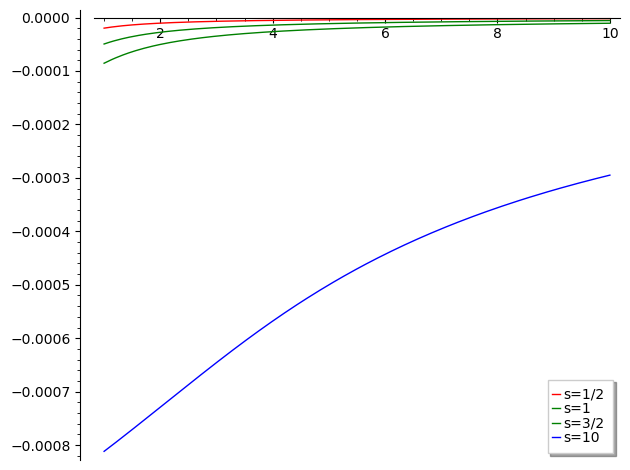
\includegraphics{figures/hw8.3.png}
\end{figure}

\end{proof}

